%marqueur aux points de données
% courbe en dessous/en dessus / intervalle dichotomie / condition d'arrêt / eps essai-erreur

Dans cette partie, nous résolvons le problème variationnel avec l'épaisseur fixée à $e=0.1$ m, à l'aide d'un programme FreeFem++.

% link free fem

\begin{problem}{3}
    Modélisons le pont et maillons-le.
\end{problem}


\begin{solution}   
    En suivant les indications de l'énoncé, nous avons commencé par réaliser les bordures, correctement "orientées" et "subdivisées", de la coupe du pont (selon l'axe $y$),
    selon la méthode vue en cours sur les maillages.%faire varier n
    Nous avons ensuite maillé la surface à l'aide de la fonction \emph{buildmesh} de FreeFem++.

    \begin{figure}[H]        
        \begin{center}
        
            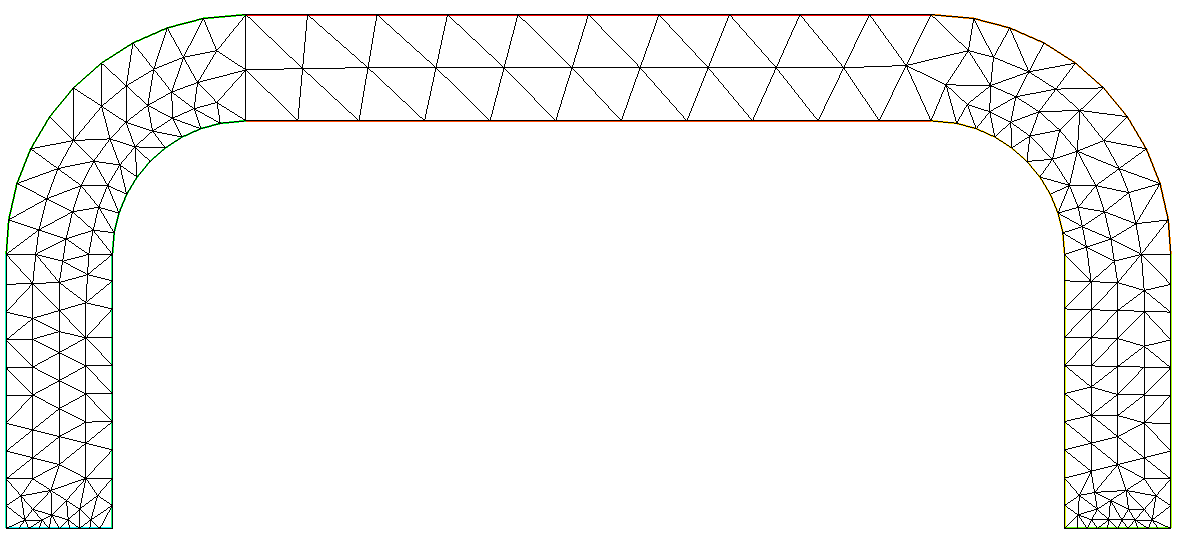
\includegraphics[width=12cm]{imgs/all_maillage_default.PNG}
            \caption{Schéma de la géométrie du pont. Une force surfacique $f= - 5x10^8 N m^(-2)$ est appliquée à sa surface supérieure. Le déplacement maximale $d$ est montré en bleue, en vert c'est $\gamma$F, surface dans lequelle la force est appliquée et $\gamma$S est la surface inférieure fixe. Le système est qui est soumis à la gravité $g$.}
            \label{fig:problem}
        
        \end{center}
    \end{figure}

    On note $n$ le paramètre contrôlant le nombre de subdivisions pour une bordure du maillage.

\end{solution}
%optimisation temps

% étude convergence